\section{Use Cases}
\label{sec:use_cases}
Due to its proximity to games and machine learning (MCTS can be viewed as a reinforcement learning algorithm) Monte Carlo Tree Search is widely applied to these two fields, some notable examples are detailed below as well as the use of MCTS in other domains. 
\subsection{Go} 
\label{ss:go}
In the machine learning research community the board game Go has long been viewed as intractable with current methods. The number of possible moves and resulting game states is much larger than Chess for example, where the average number of legal moves is $35$ with an average game length of $80$ moves, resulting in a search space of $35^{80}$ sequences. For Go we have $250$ moves, a length of $150$ and thus $250^{150}$ sequences. In a breakthrough project called AlphaGo Silver et al. \cite{silver2017mastering} combine two neural networks and MCTS to beat the European human Go champion, something that has never been done before.

\begin{figure}[ht]
    \centering
    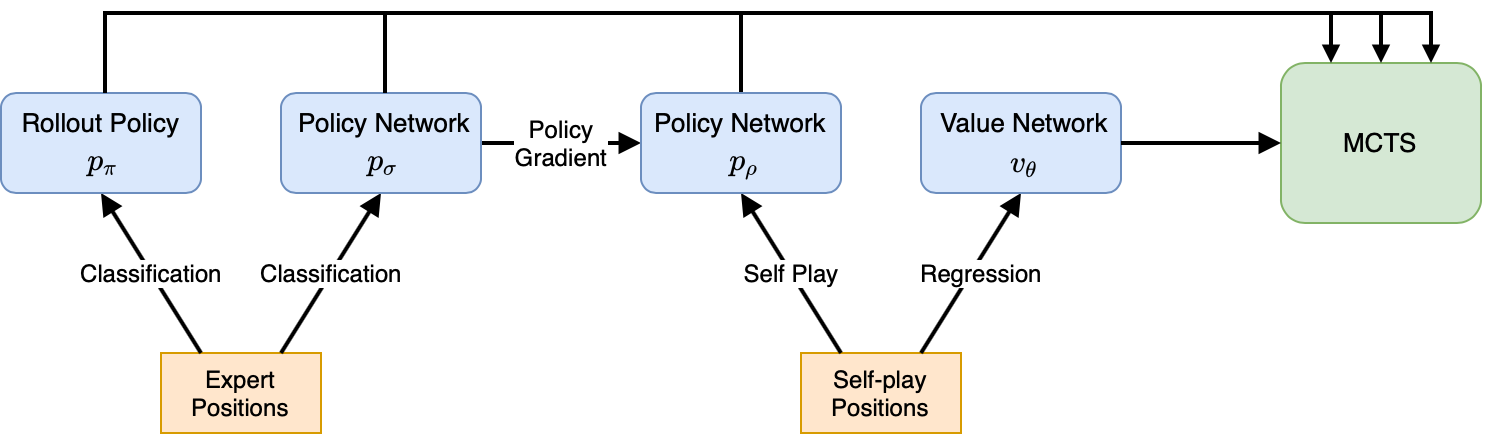
\includegraphics[width=\textwidth]{img/alphago.png}
    \caption{The basic pipeline of AlphaGo. [modified image from \cite{silver2017mastering}]}
    \label{fig:alphago}
\end{figure}

Figure \ref{fig:alphago} shows the basic steps of the approach: Initially, AlphaGo makes use of supervised learning. On the basis of input $s$ which is a simple representation of the game state a policy network outputs a probability distribution over all legal moves. This network $p_\sigma$ contains alternating convolutional layers with weights $\sigma$ and rectifier nonlinearities ending in a softmax-output layer. The concrete network used is called \textit{SL policy network} and consists of 13 layers. It was trained on 30 million positions and the associated moves of human experts, so-called state-action pairs $(s,a)$. Concretely, stochastic gradient was used to maximize the likelihood of move $a$ when in state $s$ by optimizing the following equation:
\begin{equation*}
    \frac{\partial \log p_\sigma (a | s)}{\partial \sigma}
\end{equation*}
With a less elaborate approach (a linear softmax of fewer features) another policy $p_\pi(a|s)$ was learned. This policy is far less accurate but much faster in selecting an action (2 $\mu$s compared to $3$ ms). In a second stage reinforcement learning is applied to improve the learned policy. The \textit{RL policy network} $p_\rho$ is identical in structure and (initially) has the same weights $\rho = \sigma$. This network now plays against itself, that is against randomly selected previous iterations of itself. At time step $t$ the following term is maximized (again using SGD).
\begin{equation*}
    \frac{\partial \log p_\rho(a_t | s_t)}{\partial \rho} z_t
\end{equation*}
 $z_t$ is the reward $r(s_T) \in \left\{-1,+1\right\}$ at the terminal step $T$ of the reward function $r(s)$ which is zero for any $t < T$.

In a third and final step a value network is used to estimate a value function $v^p(s)$ that predicts the outcome of games that (starting) from state $s$ are played out by using policy $p$ for both players, i.e., $v^p(s) = \mathbb{E}[z_t | s_t = s, a_t,\ldots,a_T \sim p]$. Concretely, the RP policy $p_\rho$ is estimated using a value network $v_\theta$ whose architecture is similar to that of the policy networks with weights $\theta$ but returns a single value instead of a distribution. It is trained via regression on state-outcome pairs $(s,z)$. That is the MSE between the predicted outcome $v_\theta(s)$ and the actual outcome $z$, $z-v_\theta(s)$ is minimized. MCTS is now used to combine the policy networks and the value network in a modification called \textit{lookahead search} that is similar to UCT. Exactly like in UCT each node in the search tree represents a state $s$ of the Go game and contains its incoming action $a$, its cumulative value $Q(s,a)$ and visit count $N(s,a)$. In addition it also contains the prior probability $P$ as determined by the policy network $P(s,a) = p_\sigma(a|s)$. During the simulation at step $t$ the next action is selected to maximize the term $Q(s_t,a) + u(s_t,a)$ where the latter term is a \enquote{bonus} with $u(s,a) \propto \frac{P(s,a)}{1+N(s,a)}$. When expanding a leaf node, $s_L$ is evaluated by the value network with output $v_\theta(s_L)$ and by the result $z_L$ of a simulation using $p_\pi$ as the default policy. Both these values are combined (roughly similar to (G)RAVE) using a mixing parameter $\lambda$ into a leaf evaluation $V(s_L)$ = $(1-\lambda)v_\theta(s_L)+\lambda z_L$. This value is then backpropagated. It is worth noting that this procedure uses the weaker policy $p_\sigma$ instead of the stronger policy $p_\rho$ because the former seems to be more similar to human Go-play. However, in direct competition $p_\rho$ wins 80\% of the time. 
\subsection{Neural Networks and Machine Learning}
\label{ss:nn}
\paragraph{Video Games} 
Guo et al. \cite{guo2014deep} apply an UCT-algorithm to generate training data for classifiers combining reinforcement learning and deep learning. These classifiers are then used in an AI system for playing Atari video games. For the seven games they evaluated MCTS beat the previous-state of the art AI for game playing: DQN \cite{mnih2013playing}. Concretely, the emulator for each game is accessed at a certain state yielding a deterministic Markov Decision Problem. This is then solved by UCT with 3 parameters: the number of trajectories, the maximum depth and an exploration constant. With these parameters the trajectories are simulated. Consider trajectory $k$ at state $s$ and depth $d$, i.e., the search is at the state-action pair $(s,d)$. For each possible action $a$ a score is calculated and the action with the biggest score is selected. The term to be maximized is (mostly) just a reformulation of UCT: It is the sum of the average reward of simulations in $(s,d)$ in the previous $k-1$ trajectories and the exploration term $\sqrt{\log (n(s,d)) / n(s,a,d)}$ where $n(s,a,d)$ is the number of times $a$ has been selected at $(s,d)$ and $n(s,d)$ is the total number of simulations for the previous trajectories at this pair.

To use the UCT agents in neural networks they propose three methods:
\begin{itemize}
    \item \textit{UCT to Regression}: For each game the UCT agents runs $800$ times, the dataset to train a regression-based CNN is created by saving the last four actions selected by the agents for each state and each trajectory. The result can now be viewed as a table where the rows correspond to the last four frames for each state and trajectory and the single row contains the best action (as determined by UCT).
    \item \textit{UCT to Classification}: Since the dataset above only contains a single action for each state/trajectory pair it can be easily used for classification as well with the action being the label. This is done via a CNN implementing multinomial classification.
    \item \textit{UCT to Classification Interleaved}: This method alternates data collection and playing. First the agent is run $200$ times. Now the classification is executed as above. Its results are then used to inform the agents choices in another $200$ runs, potentially leading to different results. 
\end{itemize}

Stanescu et al. \cite{stanescu2016evaluating} compare various MCTS-variations with each other as well as other search algorithms with respect to their performance in Real Time Strategy (RTS) Games and show that combining MCTS with convolutional neural networks beats many conventional state-of-the-art algorithms. To this end a simple game was designed where two players fight each other by gathering resources, creating buildings that produce units and controlling four unit types: workers, light, ranged and heavy units. Four strategies were implemented: \textit{WorkerRush} where all workers are directly sent to fight and \{Light,Ranged,Heavy\}-Rush where a barracks are built and the corresponding units are produced and sent to fight. These strategies can be viewed as actions taken by a MCTS algorithm. They introduce and compare four different variations with increasing complexity and performance:
\begin{enumerate}[label=\alph*)]
    \item \textit{Naive MCTS}: Simple MAB approach to select the action at the current game state.
    \item \textit{Greedy MCTS}: MCTS using a greedy sampling strategy (more exploitation, less exploration).
    \item \textit{AHTN-P}: An Adversarial Hierarchical Task Network using minimax gametree search as well as a RTS-variation of MCTS presented by Ontanon \cite{ontanon2013combinatorial}.
    \item \textit{AHTN-F}: A more elaborate NN using the approach above.
\end{enumerate}  
\paragraph{Deep Learning Architectures}
The problem of choosing the architecture of a neural network is critical as its performance is usually greatly affected by it. However, most research focuses on the tuning of hyperparameters, not the architecture itself resulting in a situation where the success or failure of a projects rests on intuition. To improve this process, Negrinho and Gordon \cite{negrinho2017deeparchitect} introduce a framework for the automatic generation and testing of different architectures. It consists of two parts: First, the \textit{model search specification language} allowing for the description of (complex) models, i.e., black boxes that make up parts of a neural network which are only defined by their interface (their hyperparameters) and may themselves be made up of components. Any search space defined this way will be a tree, a property used by the second component, the \textit{model search algorithm}. This algorithm determines how (and which parts of) the search space are explored. Here, a variation of MCTS is used. Its most critical subroutine is the model evaluation algorithm which determines the performance of a fully specified architecture, that is a leaf in the tree. 
\begin{figure}[ht]
    \centering
    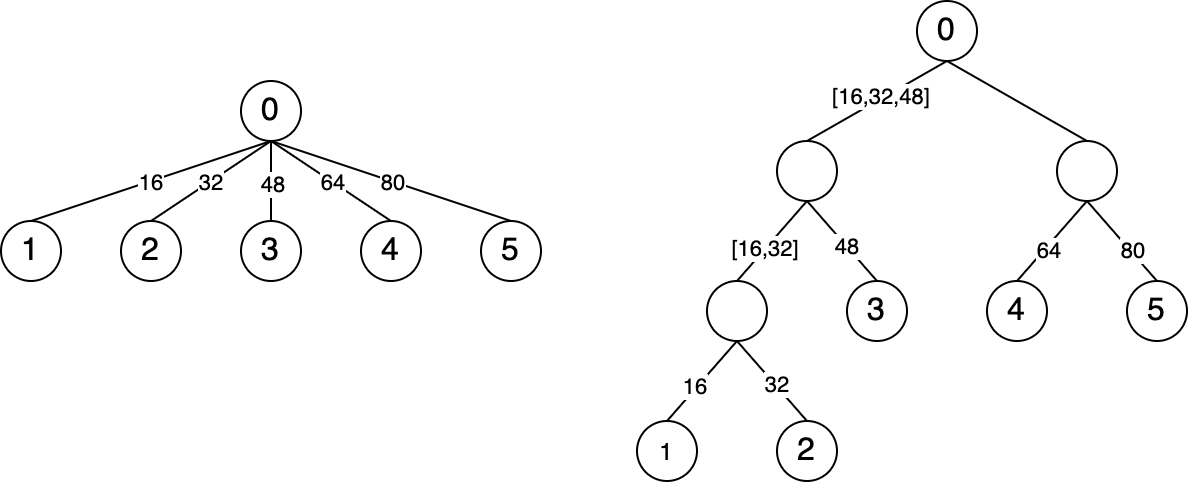
\includegraphics[width=0.9\textwidth]{img/deeparchitect.png}
    \caption{Through bisection MCTS can evaltate a large number of possible values. [modified image from \cite{negrinho2017deeparchitect}]}
    \label{fig:deep_architect}
\end{figure}
Once a search space is defined (via~a~process~not~described~here) it is explored by incrementally building a tree. The build process consists of assigning the hyperparameters of a model until it is completely specified whereby any assignment results in moving down the tree by traversing another edge. Thus, any leaf is a completely specified model and inner nodes still have unassigned parameters, the possible values of which determine the branching factor. Examples of possible assignments are integers for the number of filters of a convolutional module, or one of a relatively small set of activation functions, whether there should be a dropout layer etc. It it also important to note that (like in games) previous choices affect the number and kind of hyperparameters that are assignable later: a module that has not been selected does also need not be configured, making the path through the tree shorter.

The MCTS-algorithm used corresponds directly to UCT. The evaluation function is implemented as a machine learning prediction (i.e., as a prediction of a model trained on a training set). The default policy is simple as well, it just selects random nodes. One optimization is introduced, however. The possible values that a hyperparameter can be assigned are often numeric and thus have two properties: There are a large number of possible values but at the same time similar values are expected to yield similar performance. We can therefore make use of a bisection of the tree. Assuming a natural ordering, rather than picking a single value at a decision we choose only in which half of the set of possible values the hyperparameter will lay. This process is displayed in Figure \ref{fig:deep_architect}. One can also tune this process by experimenting with different thresholds which results in a tradeoff between breadth and depth. Experiments demonstrate that this method is superior to previous work in this area while only requiring very high-level knowledge.

Wang et al. \cite{wang2019alphax} also use MCTS in the exploration of neural network architectures in their project \textit{AlphaX}. In the benchmark suite NASBench-101 \cite{ying2019bench} their method provided a 3x speedup over simple random search. Similarly to the approach above they again define a search space of possible architectures that gets explored using Monte Carlo Tree Search. The elements of said search space are evaluated by a Meta-Deep Neural Network (DNN). While the search goes on AlphaX simultaneously generates (more) training data for the Neural Network. However, unlike in the other project there is explicit support for multiple kinds of work spaces. One of them is \textit{NASNet} where neural networks are made up of cells consisting of the layers and connections of neural networks. Like modules, they can be built recursively. The other space is called \textit{NasBench} which corresponds to a directed acyclic graph (DAG). Its nodes represent layers and its edges the connections between the layers. Since the search algorithm used is again UCB the remainder of this section focuses on the simulation step.

Generally, since neural network training is expensive (w.r.t. both time and computing resources) the actual number of times a simulation can be run is limited which decreases the accuracy of the search. To mitigate this a hybrid approach is used. The conventional training of the network is complemented by a performance prediction of the meta-DNN. This network aims to predict the performance of unseen architecture based on previously evaluated architectures as a regression task. Thus it receives a vector-representation of an architecture as input and outputs a performance metric. This encoding is rather involved but can be viewed as mapping blocks and their relations to numbers. Its training data is generated by traversing the search space. This way the Q-value of an action at a state $s$ is approximated via the following equation:
\begin{equation*}
    Q(s,a) \approx \frac{1}{2} \left(Acc(sim_0(a(s))) + \frac{1}{k} \sum_{i=1}^k Pred(sim_i(a(s))) \right)
\end{equation*} $sim_i(s)$ denotes the result of the $i$-th simulation starting from $s$, $Acc(\cdot)$ is the actual accuracy of a trained network and $Pred(\cdot)$ is the predicted accuracy of the meta-DNN.

\subsection{Other Use Cases}
\label{ss:others}
\paragraph{Databases}
Omondi \cite{omondi2019monte} applies UCT to automatically tune configuration parameters of databases. Previously these had to be manually analyzed and modified by system administrators as a reaction to environmental or runtime changes to avoid bottlenecks. The state of the database system at a point in time is quantified by measures such as the number of concurrent users, transaction throughput and the measured response time for queries. The goal of the algorithm is to optimize two of these quantities: \begin{enumerate*}[label=\roman*)]
    \item maximize the throughput, \item minimize the response time
\end{enumerate*}. Concretely, optimizing for these goals means selecting from the actions available in the current state that lead to subsequent states which perform better with respect to said goals. As described below the proposed algorithm does not actually optimize both at the same time but only one depending on the kind of database. If the workload is classified as \textit{OLTP} (Online Transaction Processing, many writes but limited reads) it is optimized w.r.t. throughput and if the workload is labeled as \textit{OLAP} (Online Analytical Processing, many reads and few writes) the goal is to minimize the response time. 

The MCTS algorithm used is a combination of UCT and a variation of a heuristic proposed by Stankiewicz \cite{stankiewicz2011monte} called \textit{Last Good Reply with Forgetting} (LGRF). The variation is called \textit{Lean LGRF}. It is used as an additional term in the UCT formula during the selection step:
\begin{equation*}
    \frac{Q(v')}{N(v')}+ LGRF_{lean}(v,v')+C_p \cdot \sqrt{\frac{2 \ln N(v)}{N(v')}}
\end{equation*}
\paragraph{Graph Matching} A (generalized) geometric graph is a tuple $G=(V,E)$ with vertices $V\subseteq \mathbb{R}^d$ and edges $E \subseteq V \times V$ where the edges are described as curves. More precisely $e \in E$ is given via a continuous function $\xi_e: [0,1] \rightarrow \mathbb{R}^d$ by $e=(\xi_e(0),\xi_e(1))$. The curve itself is the image of this function: $\xi_e(I) = \left\{\xi_e(t) | t \in I \right\}$. Intuitively, geometric graphs are regular graphs but the \enquote{actual location} of edges is defined and matters. Pinheiro et al. \cite{pinheiro2016geometric} use MCTS to define an algorithm for the problem of graph matching in this general case. The matching problem is defined as follows: Given (w.l.o.g) two graphs, determine which parts (nodes and edges) are present in both graphs. Matching of arbitrary curves can be done computationally be calculating the distance in space using some metric (e.g. Euclidean) and checking if the result is below some threshold. Clearly this is a much harder problem than matching non-geometric grahps and the well-understood theory of graph matching is not directly applicable.

Since the relationship between curves of different graphs is not immediately clear (that is, two curves in one graph may correspond to only one in the other) the concept of superedges is used. A superedge $s=(e_1,e_k)$ consists of a sequence of $k$ edges, its corresponding curve $\xi_s$ is the concatenation of the curves $\xi_{e_1},\ldots\xi_{e_k}$. For a graph $G$ let $S$ denote the set of all its superedges. Then, a matching $M$ between two geometric graphs $G_1,G_2$ can be defined as a set of superedge pairs $M \subseteq S_1 \times S_2$. The quality $Q$ of a matching $M$ consisting of a node matching $M^V$ and an superedge matching $M^S$ between graphs $G_1,G_2$ can be evaluated using the equation $Q(M^V,M^S) = l(M^S) + \kappa \ \overline{l(S_1,S_2)} \ \left| M^V \right|$ where $l(M^S)$ is the sum of the length of the edges that are members of the superedges and $\overline{l(S_1,S_2)}$ is the average length of the superedges of both graphs and $\kappa > 0$ is a constant set to $0.8$ in the algorithm below. The proposed MCTS algorithm is illustrated in Figure \ref{fig:matching}. It starts with an empty matching and in each step adds a superedge pair. For the child selection a variant of UCT is used by maximizing the equation:
\begin{equation*}
    \frac{Q(v')}{Q_{norm}(v')}+C_p \cdot \sqrt{\frac{2 \ln N(v)}{N(v')}}
\end{equation*} The denominator $Q_{norm}(\cdot)$ is a normalization factor and upper bound for the node reward $Q(v')$.
\begin{figure}[ht]
    \centering
    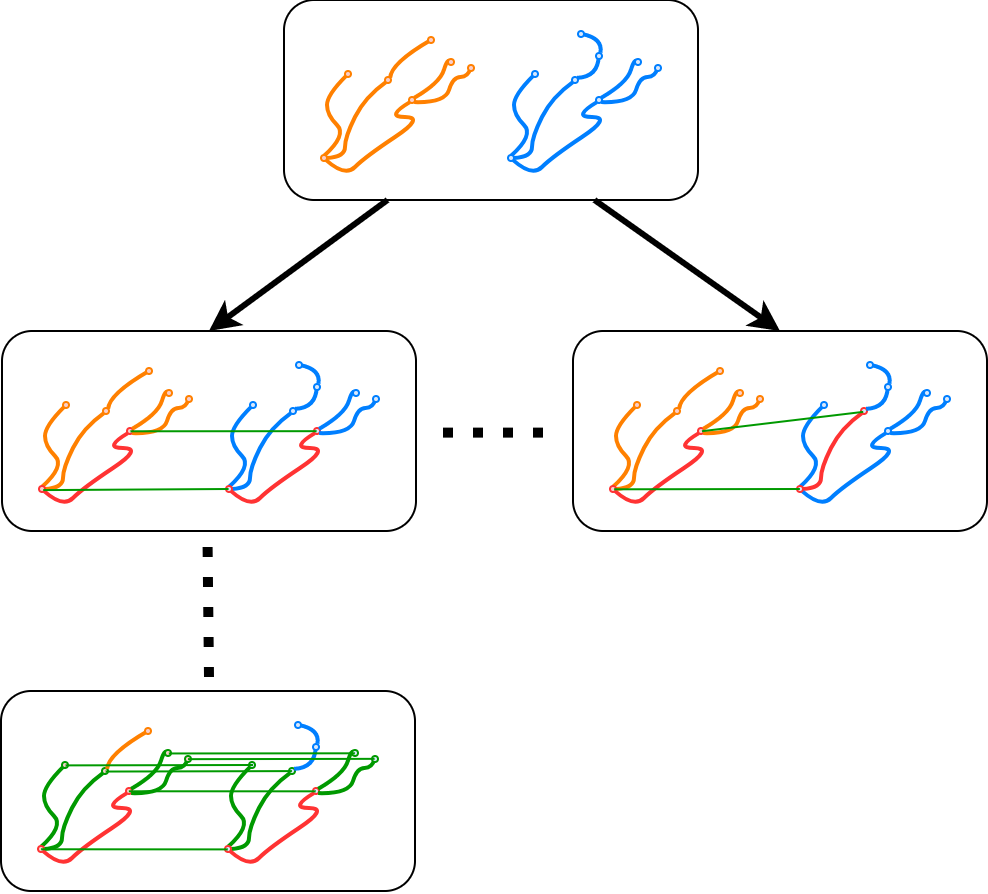
\includegraphics[width=0.6\textwidth]{img/matching.png}
    \caption{The MCTS matching algorithm. Different actions lead to selecting different superedges. The simulation result displayed is the optimal matching for the given graphs. [modified image from \cite{pinheiro2016geometric}]}
    \label{fig:matching}
\end{figure}
\FloatBarrier